\section{Luthfi Muhammad Nabil (1174035)}

\subsection{Teori}
\begin{enumerate}
    \item Jelaskan apa itu klasifikasi teks, sertakan gambar illustrasi buatan sendiri. \par
    Klasifikasi teks merupakan sebuah metode untuk memilah setiap kata yang ada dan mengelompokkannya berdasarkan kelompok yang telah ditentukan. Seperti halnya pengelompokkan surat ke kategori spam atau sms, memfilter berita sesuai kategori yang ada. Biasanya klasifikasi teks digunakan untuk memfilter dan mengelompokkan banyak konten menjadi beberapa yang dapat dibedakan berdasarkan kelompok yang sudah ditentukan. Untuk contoh penyaringan yaitu jika ada sekitar sekian persen isi dari konten didominasi dengan kategori tertentu (Misal : Komputer), maka konten yang dikirim merupakan konten dengan tema komputer.
    \begin{figure}[ht]
        \centering
        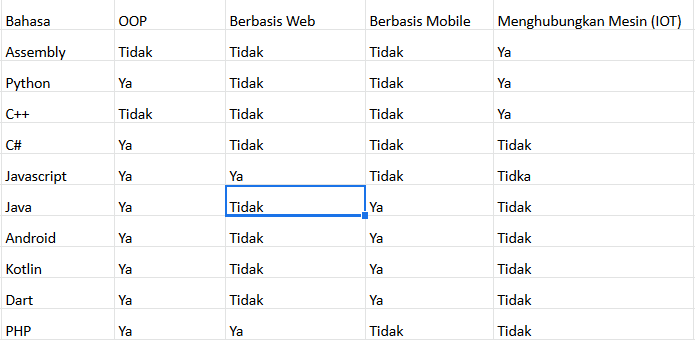
\includegraphics[scale=0.2]{figures/1174035/chapter4/1_teori.png}
        \caption{Illustrasi Klasifikasi Teks}
        \label{contoh1}
    \end{figure}
    \item Jelaskan mengapa klasifikasi bunga tidak bisa menggunakan machine learning, sertakan illustrasi sendiri \par 
    Klasifikasi bunga tidak dapat menggunakan metode machine learning karena banyaknya jenis - jenis dari bunga yang sama namun makna dari bunga tersebut dapat berbeda - beda. Sehingga akan membingungkan sebuah mesin saat memfilter data yang ada. Jika ada pun akan terjadi ketidak tepatan data karena ciri - ciri dari sebuah bunga yang dominan hampir mirip bahkan bisa sama namun dengan makna yang berbeda - beda. 
    \begin{figure}[ht]
        \centering
        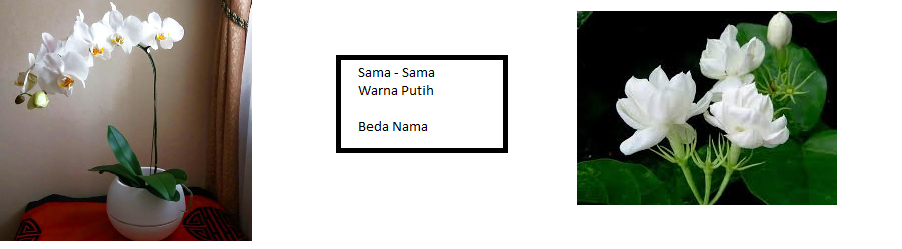
\includegraphics[scale=0.2]{figures/1174035/chapter4/2_teori.png}
        \caption{Maksud klasifikasi bunga tidak bisa}
        \label{contoh2}
    \end{figure}
    \item Jelaskan bagaimana teknik pembelajaran mesin pada teks pada kata-kata yang digunakan di youtube, jelaskan arti per atribut data csv dan sertakan illustrasi buatan sendiri \par
    Cara youtube mempelajari pemecahan teks untuk dapat membedakan mana yang merupakan sebuah kategori yaitu mengelompokkan kandidat - kandidat yang dimiliki untuk dapat ditampilkan pada user tersebut. Dimulai dari dimana user tinggal, ranking video berdasarkan daerah, riwayat dari pencarian user, dan lain sebagainya. Saat user menginputkan sebuah pencarian, youtube akan merekam pencarian tersebut untuk menjadikan referensi dari apa yang pengguna sering cari sehingga tau apa konteks dari yang dicari pengguna tersebut. Hal itu dilakukan karena terkadang satu kata memiliki banyak makna sehingga youtube akan menyesuaikan makna yang dicari dengan apa yang dimaksud dengan user tersebut. 
    \begin{figure}[ht]
        \centering
        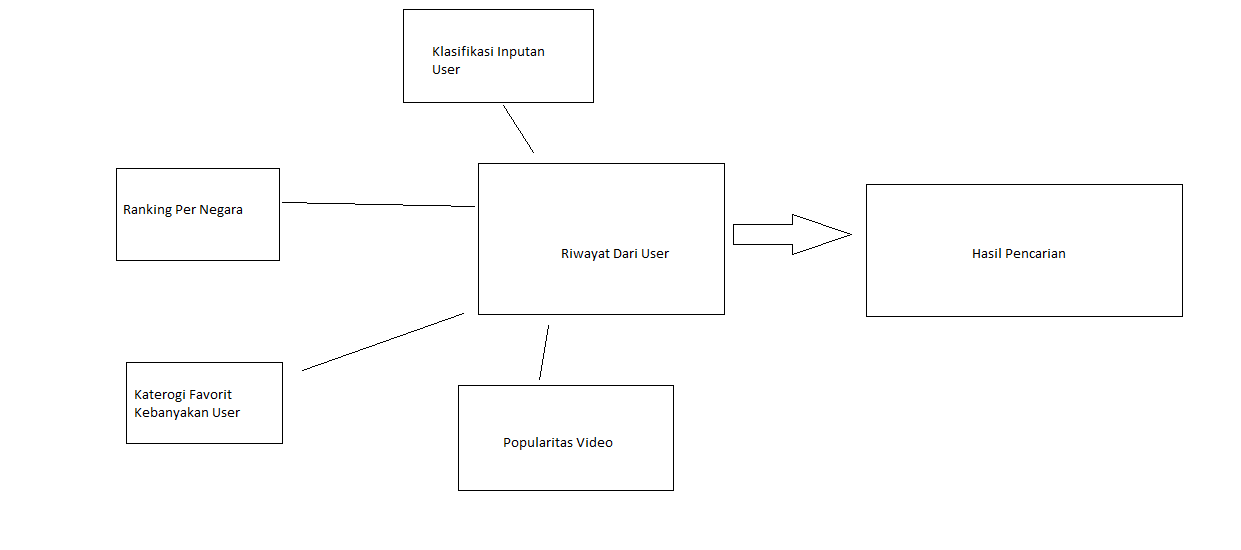
\includegraphics[scale=0.2]{figures/1174035/chapter4/3_teori.png}
        \caption{Teknik filtering pada youtube}
        \label{contoh3}
    \end{figure}
    \item Jelaskan apa yang dimaksud vektorisasi data \par
    Vektorisasi data merupakan proses konversi data raster yang diubah menjadi data vektor. Parameter yang digunakan biasanya berupa data beberapa persentase atau kondisi ya/tidak yang berbentuk numerik untuk membedakan setiap data itu memiliki makna apa pada parameter yang dimaksud. Konversi itu wujudnya disebut digitasi. Vektorisasi data perlu dilakukan karena untuk menghitung sebuah nilai pada Artificial Intelligence, diperlukan angka yang dapat dihitung dan kategori dari nilai tersebut sehingga memudahkan dalam menghitung dan menentukan apa yang perlu dilakukan.
    \item Jelaskan apa itu bag of words dengan kata-kata yang sederhana dan illustrasi sendiri. \par
    Bag of Words merupakan model representasi sederhana yang dipakai untuk pengambilan informasi dan pemrosesan bahasa umum atau alami. Pada model ini, sebuah teks akan dikategorikan sebagai bungkusan dari kumpulan kata tanpa perlu diolah ulang sekalipun. Bag of words juga digunakan pada klasifikasi dokumen yang biasanya setiap kata digunakan sebagai fitur dari pelatihan klasifikasi. 
    \begin{figure}[ht]
        \centering
        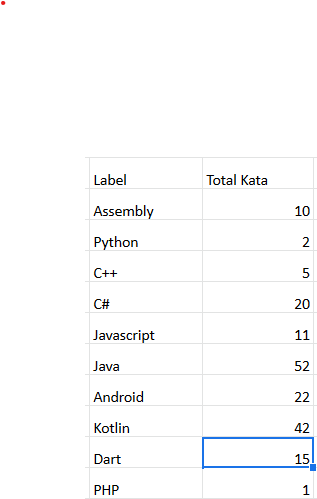
\includegraphics[scale=0.2]{figures/1174035/chapter4/5_teori.png}
        \caption{Illustrasi Bag of Words}
        \label{contoh4}
    \end{figure}
    \item Jelaskan apa itu TF-IDF, illustrasikan dengan gambar sendiri..
    TF-IDF merupakan pengukuran statistik yang mengevaluasi seberapa bernilai kata yang dicek di dalam dokumen tersebut. Parameter yang digunakan biasanya yaitu berapa banyak kata tersebut muncul pada sebuah dokumen. Biasanya metode ini digunakan untuk menilai sebuah kata yang digunakan pada algoritma machine learning.
    \begin{figure}[ht]
        \centering
        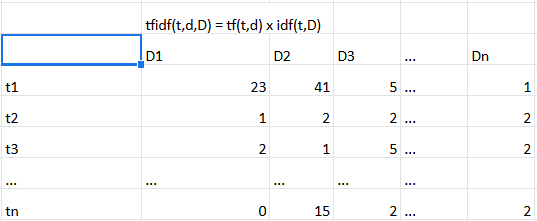
\includegraphics[scale=0.2]{figures/1174035/chapter4/6_teori.png}
        \caption{Illustrasi TF-IDF}
        \label{contoh5}
    \end{figure}
\end{enumerate}

\subsection{Praktek}
\begin{enumerate}
    \item Buat aplikasi sederhana menggunakan pandas, buat data dummy format csv sebanyak 500 baris dan melakukan load ke dataframe pandas. Jelaskan arti setiap baris kode yang dibuat.
    \lstinputlisting[firstline=1, lastline=11]{src/1174035/chapter4/1_praktek.py}
    \item Dari dataframe tersebut, dipecah menjadi dua dataframe yaitu 450 row pertama dan 50 row sisanya(Harus beda dengan teman sekelas)
    \lstinputlisting[firstline=12]{src/1174035/chapter4/1_praktek.py}
    \item Praktekkan vektorisasi dan klasifikasi dari data Shakira dengan decision tree. Tunjukkan keluarannya dari komputer sendiri dan artikan maksud dari setiap luaran yang didapatkan.
    \lstinputlisting[firstline=8, lastline=49]{src/1174035/chapter4/3_praktek.py}
    \begin{figure}[ht]
        \centering
        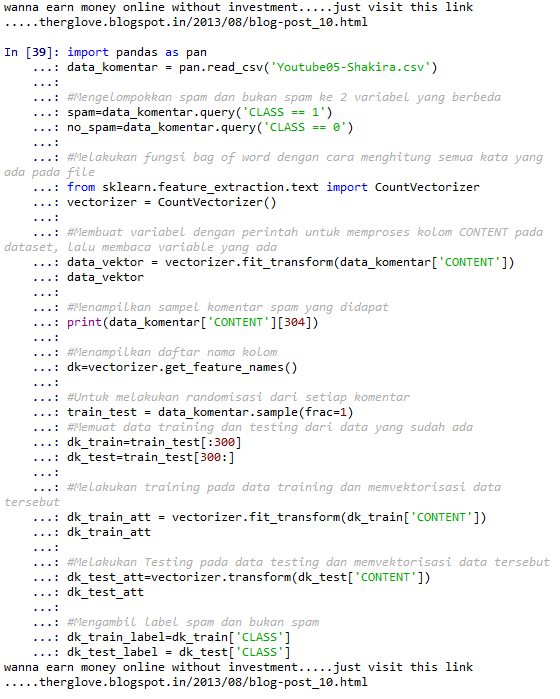
\includegraphics[scale=0.2]{figures/1174035/chapter4/3_praktek.png}
        \caption{Melakukan vektorisasi dan mengambil salah satu contoh}
        \label{contoh6}
    \end{figure}
    \item Cobalah klasifikasikan dari data vektorisasi yang ditentukan di nomor sebelumnya dengan klasifikasi SVM. Tunjukkan keluarannya dari komputer sendiri dan artikan maksud setiap luaran yang didapatkan.
    \lstinputlisting[firstline=53, lastline=57]{src/1174035/chapter4/3_praktek.py}
    \begin{figure}[ht]
        \centering
        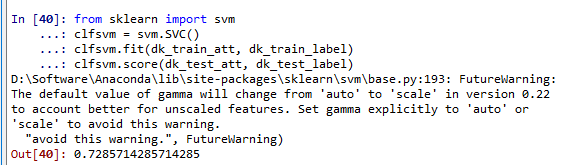
\includegraphics[scale=0.2]{figures/1174035/chapter4/4_praktek.png}
        \caption{Melakukan prediksi CVM berdasarkan nilai}
        \label{contoh7}
    \end{figure}
    \item Coba klasifikasikan dari data vektorisasi yang ditentukan di nomor sebelumnya dengan klasifikasi Decision Tree. Tunjukkan kelaurannya dari komputer sendiri dan artikan maksud setiap luaran yang didapatkan.
    \lstinputlisting[firstline=60, lastline=64]{src/1174035/chapter4/3_praktek.py}
    \begin{figure}[ht]
        \centering
        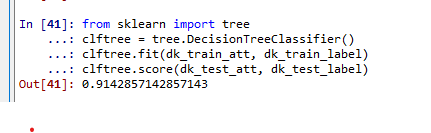
\includegraphics[scale=0.2]{figures/1174035/chapter4/5_praktek.png}
        \caption{Klasifikasi data dari vektorisasi yang ada dengan decision tree}
        \label{contoh8}
    \end{figure}
    \item Plotlah confusion matrix dari praktek modul ini menggunakan matplotlib. Tunjukkan keluarannya dari komputer sendiri dan artikan maksud setiap luaran yang didapatkan
    \lstinputlisting[firstline=66, lastline=72]{src/1174035/chapter4/3_praktek.py}
    \begin{figure}[ht]
        \centering
        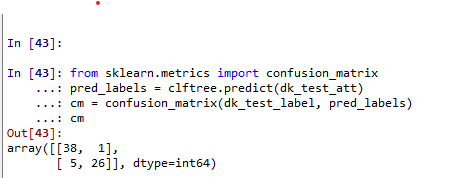
\includegraphics[scale=0.2]{figures/1174035/chapter4/6_praktek.png}
        \caption{Penggunaan confusion matrix}
        \label{contoh9}
    \end{figure}
    \item Jalankan program cross validation pada bagian teori bab ini. Tunjukkan keluarannya dari komputer sendiri dan artikan mnaksud setiap luaran yang didapatkan.
    \lstinputlisting[firstline=74, lastline=90]{src/1174035/chapter4/3_praktek.py}
    \begin{figure}[ht]
        \centering
        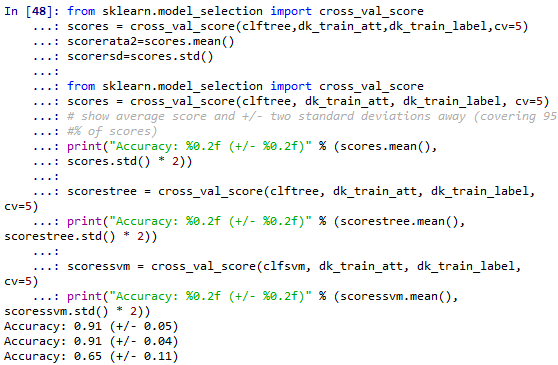
\includegraphics[scale=0.2]{figures/1174035/chapter4/7_praktek.png}
        \caption{Mengambil tingkat akurasi dari klasifikasi data dan prediksi}
        \label{contoh11}
    \end{figure}
    \item Buatlah program pengamatan komponen informasi pada bagian teori bab ini. Tunjukkan keluarannya dari komputer sendiri dan artikan maksud setiap luaran yang didapatkan
    \lstinputlisting[firstline=91]{src/1174035/chapter4/3_praktek.py}
    \begin{figure}[ht]
        \centering
        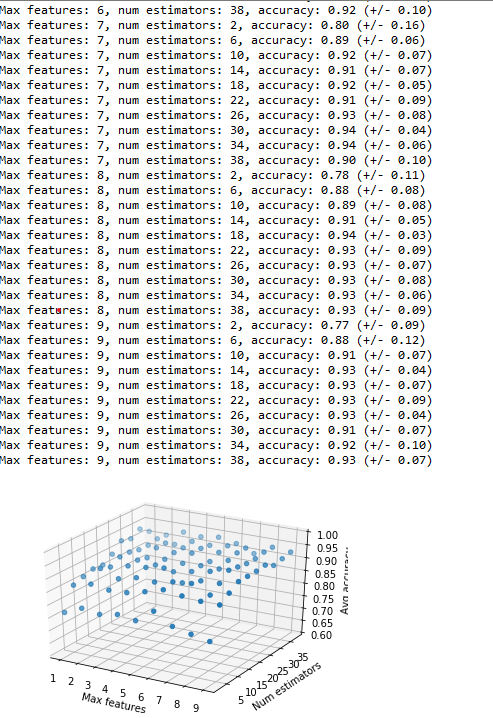
\includegraphics[scale=0.2]{figures/1174035/chapter4/8_praktek.png}
        \caption{Melakukan regresi data dengan numpy dan mengambil fitur - fitur yang ada}
        \label{contoh12}
    \end{figure}
\end{enumerate}
\subsection{Penanganan Error}
\begin{enumerate}
    \item Skrinsut Error
    \begin{figure}[ht]
        \centering
        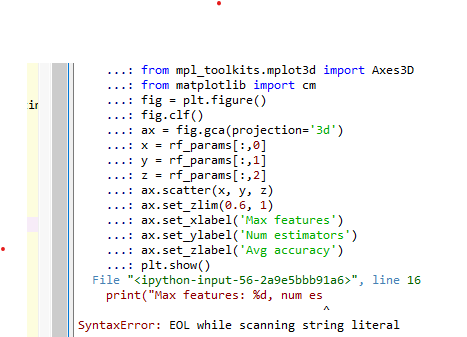
\includegraphics[scale=0.2]{figures/1174035/chapter4/error.png}
        \caption{Error}
        \label{contoh13}
    \end{figure}
    \item Tipe Error : EOF
    \item Penanganan : Meluruskan String
    \begin{verbatim}
        #Awalnya
        print("Max 
        features: %d, num estimators: %d, accuracy: %0.2f (+/- %0.2f)" 
        #Sekarang
        print("Max features: %d, num estimators: %d, accuracy: %0.2f (+/- %0.2f)" 
    \end{verbatim}
\end{enumerate}
